\documentclass[10pt]{article}
\usepackage[polish]{babel}
\usepackage[utf8]{inputenc}
\usepackage[T1]{fontenc}
\usepackage{graphicx}
\usepackage[export]{adjustbox}
\graphicspath{ {./images/} }
\usepackage{amsmath}
\usepackage{amsfonts}
\usepackage{amssymb}
\usepackage[version=4]{mhchem}
\usepackage{stmaryrd}

\newcommand\Varangle{\mathop{{<\!\!\!\!\!\text{\small)}}\:}\nolimits}

\begin{document}
\begin{enumerate}
  \item Czworokąt wypukły ABCD, nie będący trapezem, jest wpisany w okrąg. Półproste AB i DC przecinają się w punkcie M , a półproste DA i CB przecinają się w punkcie N. Wyznaczyć kąty czworokąta ABCD, jeżeli\\
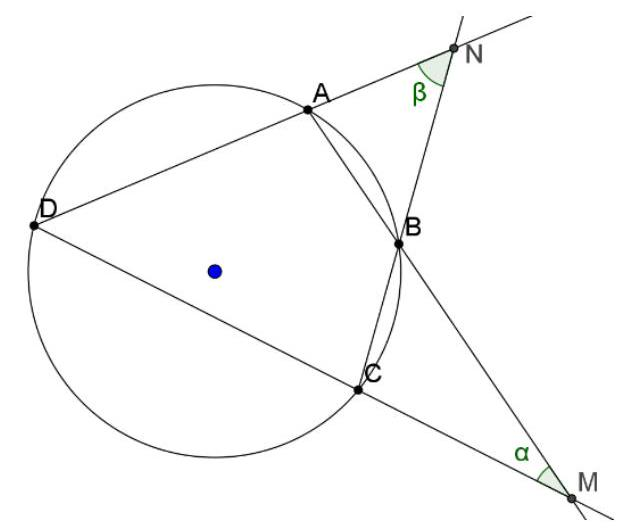
\includegraphics[max width=\textwidth, center]{2024_11_21_541d3b47acfc0b787715g-1(1)}\\
\(\Varangle B M C=\alpha \mathrm{i} \Varangle A N B=\beta\)
  \item Dany jest trójkąt ABC o kącie prostym przy wierzchołku C.\\
Dwusieczne kątów przy\\
wierzchołkach A i B przecinają boki\\
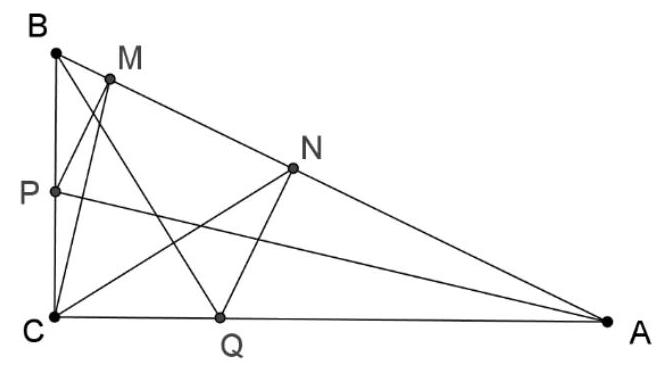
\includegraphics[max width=\textwidth, center]{2024_11_21_541d3b47acfc0b787715g-1}\\
trójkąta odpowiednio w punktach Pi Q. Niech M i N będą rzutami prostopadłymi punktów P i Q na bok AB. Znaleźć miarę kąta MCN.
\end{enumerate}

Wyznacz liczbę par \((x, y)\) liczb całkowitych spełniających równanie \(x^{4}=y^{4}+1223334444\).


\end{document}